%!TEX program = xelatex
\documentclass[10pt]{article}
\usepackage{amssymb}
\usepackage{amsmath}
\usepackage{mathrsfs}
\usepackage{titlesec}
\usepackage{xcolor}
\usepackage{enumerate}
\usepackage{bm}
\usepackage{tikz}
\usepackage{listings}
\usetikzlibrary{arrows}
\usepackage{subfigure}
\usepackage{graphicx,booktabs,multirow}
\usepackage[a4paper]{geometry}
\usepackage{upquote}
\usepackage{float}
\usepackage{pdfpages}

\geometry{verbose,tmargin=2cm,bmargin=2cm,lmargin=2cm,rmargin=2cm}
\geometry{verbose,tmargin=2cm,bmargin=2cm,lmargin=2cm,rmargin=2cm}
\lstset{language=Matlab}
\lstset{breaklines}

\input defs.tex

\newtheorem{proposition}{Proposition}
\newtheorem{remark}{Remark}

\titleformat*{\section}{\centering\LARGE\scshape}
\renewcommand{\thesection}{\Roman{section}}
\lstset{language=Matlab,tabsize=4,frame=shadowbox,basicstyle=\footnotesize,
keywordstyle=\color{blue!90}\bfseries,breaklines=true,commentstyle=\color[RGB]{50,50,50},stringstyle=\ttfamily,numbers=left,numberstyle=\tiny,
  numberstyle={\color[RGB]{192,92,92}\tiny},backgroundcolor=\color[RGB]{245,245,244},inputpath=code}

\begin{document}

\date{\today}
\title{Introduction to Machine Learning, Spring 2023 \\
	Homework 2\\
	\small (Due Thurs, Mar. 23 at 11:59pm (CST))}
\maketitle
\begin{enumerate}[1.]


\item \defpoints{15}
Kernel functions implicitly define some mapping function  $\phi(\cdot)$  that transforms an input instance  $\mathbf{x} \in \mathbb{R}^{d}$  to high dimensional space  Q  by giving the form of dot product in  Q: $K\left(\mathbf{x}_{i}, \mathbf{x}_{j}\right) \equiv   \left\langle\phi\left(\mathbf{x}_{i}\right), \phi\left(\mathbf{x}_{j}\right)\right\rangle $
\begin{itemize}
    \item[(a)]  Prove that the kernel is symmetric,i.e. $K\left(\mathbf{x}_{i}, \mathbf{x}_{j}\right)=K\left(\mathbf{x}_{j}, \mathbf{x}_{i}\right).$\defpoints{5}
    \\
    \textcolor{blue}{solution: As the the kernel function is defined as $$K\left(\mathbf{x}_{i}, \mathbf{x}_{j}\right) \equiv   \left\langle\phi\left(\mathbf{x}_{i}\right), \phi\left(\mathbf{x}_{j}\right)\right\rangle $$
    Then we have that for any two input mapping function $\phi\left(\mathbf{x}_{i}\right), \phi\left(\mathbf{x}_{j}\right) \in R$, then we use the property of dot product, we have that $$K\left(\mathbf{x}_{i}, \mathbf{x}_{j}\right)\equiv\left\langle\phi\left(\mathbf{x}_{i}\right), \phi\left(\mathbf{x}_{j}\right)\right\rangle \equiv \left\langle\phi\left(\mathbf{x}_{j}\right), \phi\left(\mathbf{x}_{i}\right)\right\rangle \equiv K\left(\mathbf{x}_{j}, \mathbf{x}_{i}\right)$$
    So we get that the kernel is symmetric.}
 \item[(b)] Assume we use radial basis kernel function  $K\left(\mathbf{x}_{i}, \mathbf{x}_{j}\right)=\exp \left(-\frac{1}{2}\left\|\mathbf{x}_{i}-\mathbf{x}_{j}\right\|^{2}\right)$. Thus there is some implicit unknown mapping function  $\phi(\mathbf{x}) $. Prove that for any two input instances  $\mathbf{x}_{i}$  and  $\mathbf{x}_{j}$, the squared Euclidean distance of their corresponding points in the feature space  Q  is less than 2, i.e. prove that  $\left\|\phi\left(\mathbf{x}_{i}\right)-\phi\left(\mathbf{x}_{j}\right)\right\|^{2} \leq 2$.\defpoints{5}

\textcolor{blue}{solution: the radial basis kernel function is defined as $$K\left(\mathbf{x}_{i}, \mathbf{x}_{j}\right)=\exp \left(-\frac{1}{2}\left\|\mathbf{x}_{i}-\mathbf{x}_{j}\right\|^{2}\right)$$
    Then we have that $$\parallel\phi(\mathbf{x}_{i}) - \phi(\mathbf{x}_{j})\parallel^2 = $$}

\item[(c)] With the help of a kernel function, SVM attempts to construct a hyper-plane in the feature space  Q  that maximizes the margin between two classes. The classification decision of any  $\mathbf{x}$  is made on the basis of the sign of$$
\langle\hat{\mathbf{w}}, \phi(\mathbf{x})\rangle+\hat{w}_0=\sum_{i \in S V} y_i \alpha_i K\left(\mathbf{x}_i, \mathbf{x}\right)+\hat{w}_0=f\left(\mathbf{x} ; \alpha, \hat{w}_0\right),
$$
where $\hat{\mathbf{w}}$ and $\hat{w}_0$ are parameters for the classification hyper-plane in the feature space $Q, S V$ is the set of support vectors, and $\alpha_i$ is the coefficient for the $i$-th support vector. Again we use the radial basis kernel function. Assume that the training instances are linearly separable in the feature space $Q$, and assume that the SVM finds a margin that perfectly separates the points.

If we choose a test point $\mathbf{x}_{f a r}$ which is far away from any training instance $\mathbf{x}_i$ (distance here is measured in the original space $\left.\mathbb{R}^d\right)$, prove that $f\left(\mathbf{x}_{f a r} ; \alpha, \hat{w}_0\right) \approx \hat{w}_0$.\defpoints{5}
\\
\textcolor{blue}{solution:}

\end{itemize}
\newpage
\item \defpoints{15}The Poisson distribution is a useful discrete distribution which can be used to model the number of occurrences of something per unit time. For example, in networking, the number of packets to arrive in a given time window is often assumed to follow a Poisson distribution. If $X$ is Poisson distributed, i.e. $X \sim \operatorname{Poisson}(\lambda)$, its probability mass function takes the following form:
$$
P(X \mid \lambda)=\frac{\lambda^x e^{-\lambda}}{X !}
$$
It can be shown that if $\mathbb{E}(X)=\lambda$. Assume now we have $n$ i.i.d. data points from Poisson $(\lambda)$ : $\mathcal{D}=\left\{X_1, \ldots, X_n\right\}$
(For the purpose of this problem, you can only use the knowledge about the Poisson and Gamma distributions provided in this problem.)
\item[(a)] Show that the sample mean $\hat{\lambda}=\frac{1}{n} \sum_{i=1}^n X_i$ is the maximum likelihood estimate (MLE) of $\lambda$ and it is unbiased $(\mathbb{E}(\hat{\lambda})=\lambda)$. \defpoints{5}
\\
\textcolor{blue}{solution:}


\item[(b)]Now let's be Bayesian and put a prior distribution over $\lambda$. Assuming that $\lambda$ follows a Gamma distribution with the parameters $(\alpha, \beta)$, its probability density function:
$$
p(\lambda \mid \alpha, \beta)=\frac{\beta^\alpha}{\Gamma(\alpha)} \lambda^{\alpha-1} e^{-\beta \lambda}
$$
where $\Gamma(\alpha)=(\alpha-1)$ ! (here we assume $\alpha$ is a positive integer). Compute the posterior distribution over $\lambda$. \defpoints{5}
\\
\textcolor{blue}{solution:}
\item[(c)] Derive an analytic expression for the maximum a posterior (MAP) of $\lambda$ under Gamma $(\alpha, \beta)$ prior.\defpoints{5}
\\
\textcolor{blue}{solution:}




\newpage
\item \defpoints{10} using d-separation on figure\ref{bayesnet} to discuss the following questions.
\begin{figure}[htbp]
    \centering
    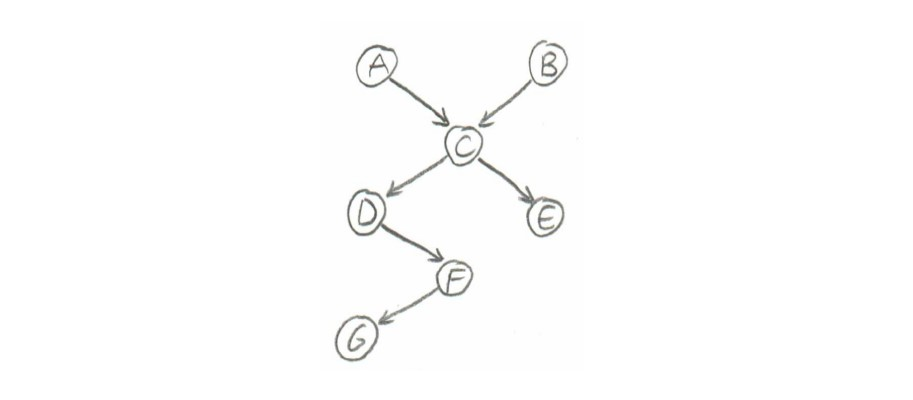
\includegraphics[scale=0.5]{figs/p3_1.jpg}
    \caption{A Bayes net}
    \label{bayesnet}
    \end{figure} 

\item[(a)] Are A and B conditionally independent, given D and F? \defpoints{5}

    \textcolor{blue}{solution:}

\item[(b)] $P(D|CEG) =? P(D|C)$\defpoints{5}

\textcolor{blue}{solution:}
\end{enumerate}

\end{document}